\documentclass[tikz]{standalone}

\usepackage{tikz}
\usetikzlibrary{intersections, patterns, calc}
\usepackage{pgfplots}
\usepgfplotslibrary{fillbetween}
\pgfplotsset{compat=newest}

\begin{document}
	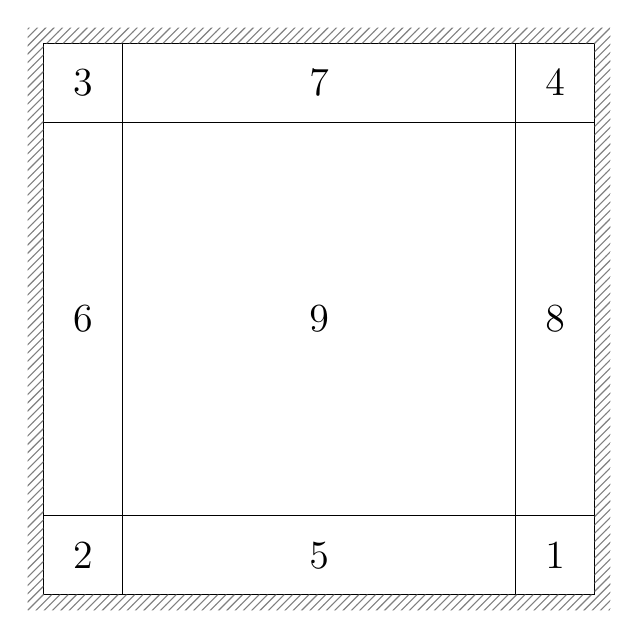
\begin{tikzpicture}
		\pgfdeclarelayer{ft}
		\pgfsetlayers{main,ft}

		\pgfmathsetmacro{\wallwidth}{0.2}

		\pgfmathsetmacro{\size}{7}
		
		\draw[name path=internal] (0,0) rectangle (\size,\size);
		\path[name path=external] (-\wallwidth, -\wallwidth) rectangle (\size + \wallwidth, \size + \wallwidth);
		\tikzfillbetween[of=external and internal, on layer=ft] {pattern=north east lines, pattern color=black!50!white}
		\foreach \x/\y[count=\i] in {2/0, 0/0, 0/2, 2/2, 1/0, 0/1, 1/2, 2/1, 1/1}
		{
			%\draw (3 * \x, 3 * \y) rectangle (3 * \x + 1, 3 * \y + 1);
			\node (state\i) at ($(3 * \x, 3 * \y) + (0.5, 0.5)$) {\Large \i};
		}		

		% draw 4 lines
		\draw (0, 1) -- +(\size, 0);
		\draw (0, \size - 1) -- +(\size, 0);
		\draw (1, 0) -- + (0, \size);
		\draw (\size - 1, 0) -- + (0, \size);
	\end{tikzpicture}
\end{document}
